\ifdefined\COMPILINGMAIN
% Main file is compiling this section, skip the preamble
\else
% Individual file compilation
\documentclass[11pt]{article}
% Geometry and page layout
\usepackage{geometry}
\geometry{verbose,tmargin=3.375cm,bmargin=2cm,lmargin=3.375cm,rmargin=3.375cm}

% Input encoding and font settings
\usepackage[utf8]{inputenc}

% other fonts
%Slightly more bold
% \usepackage{mlmodern}
% \usepackage[T1]{fontenc}

%Moder modern look
% \usepackage{libertine}
% \usepackage{libertinust1math}
% \usepackage[T1]{fontenc}

\usepackage{amsfonts, amsmath, amsthm, bbm, setspace}
\onehalfspacing
\usepackage{algorithm2e}
\usepackage{tcolorbox} % For the grey background
% Create a tcolorbox style for the algorithm
\tcbuselibrary{listingsutf8}
\tcbset{
    algobox/.style={
        colback=gray!3, % Background color
        colframe=black,  % Border color
        sharp corners,   % Square corners
        boxrule=0.5pt,   % Border thickness
        before skip=10pt, % Vertical spacing before box
        after skip=10pt,  % Vertical spacing after box
        width=\textwidth, % Box width
    }
}

% Adjust algorithm2e settings for a similar look
\SetKwInOut{Input}{Input}
\SetKwInOut{Result}{Result}
\SetKwFor{For}{for}{:}{end}

% Adjust settings for algorithm2e
\SetAlgoCaptionSeparator{.} % Separator for caption
\SetAlgoNlRelativeSize{-2}  % Adjust line number font size
\SetAlgoInsideSkip{2pt}    % Reduce space between lines
\SetAlCapSkip{0pt}         % Remove extra space after the caption
% Ensure captions are above algorithms
\SetAlgoCaptionLayout{center} % Center caption
% Adjust the style of the algorithm to remove bottom line
\RestyleAlgo{ruled}
\SetAlCapSkip{0.5em}       % Space after caption
\SetAlgoVlined              % Ensures no horizontal lines at the end

% Theorem and math environments
\newtheorem{assumption}{Assumption}
\newtheorem{lemma}{Lemma}
\newtheorem{theorem}{Theorem}

% New math commands
\newcommand{\npsym}{\mathrel{\ooalign{\raisebox{.6ex}{$>$}\cr\raisebox{-.6ex}{$<$}}}}

% Table formatting
\usepackage{booktabs, multirow, array, tabularx}
\newcolumntype{N}{>{\centering\arraybackslash}m{.85in}}

% Caption settings
\usepackage{caption}
\captionsetup{format=plain, font=footnotesize, labelfont=bf,width=3.5in}
\setlength{\abovecaptionskip}{3pt plus 3pt minus 3pt}

% Figures and floats setup
\usepackage{graphicx, adjustbox,subcaption}
\usepackage{floatrow}
\floatsetup[figure]{capposition=top}
\floatsetup[table]{capposition=top}
\renewcommand\thefigure{\thesection.\arabic{figure}}
% Path to figures
\graphicspath{{../Figures/}}
\usepackage{tikz} % TikZ for creating figures
% URLs and references and colors
\usepackage[dvipsnames]{xcolor}
\usepackage[hyphens]{url}
\usepackage{hyperref}
\hypersetup{
    colorlinks=true,
    citecolor=[HTML]{901A1E}, %KU red
    linkcolor=[HTML]{901A1E}, %KU red    
    filecolor=blue, 
    urlcolor=[HTML]{901A1E}, %KU red
    hyperindex=true,
    hyperfigures=true,
    hyperfootnotes=true,
}

% Biblatex settings for references
\usepackage[style=authoryear, dashed=false, backend=bibtex]{biblatex}
\addbibresource{../Ref.bib}

\renewbibmacro*{volume+number+eid}{%
  \printfield{volume}%
  \setunit*{\addcomma\space}%
  \printfield{number}%
  \setunit{\addcomma\space}%
  \printfield{eid}
}
\DeclareFieldFormat[article]{volume}{\bibstring{volume}~#1}
\DeclareFieldFormat[article]{number}{\bibstring{number}~#1}
\DefineBibliographyStrings{english}{volume = {Vol.}, number = {No.}}

% Author name formatting
\DeclareNameAlias{author}{last-first}
\renewcommand*{\finalnamedelim}{\addspace and\space}
\renewcommand*{\multinamedelim}{\addcomma\space}

% Footnotes and appendix setup
\usepackage[hang,flushmargin]{footmisc}
\usepackage[toc,page]{appendix}
\renewcommand\appendixtocname{Appendices}
\renewcommand\appendixpagename{Appendices}

%# Assumptions like theorems and corrolaries
% {
%   \theoremstyle{plain}
%   \newtheorem{assumption}{Assumption}
% }
% Title setup
\usepackage{titlepic}
\usepackage{titlesec}
\titleformat{\section}{\normalfont\Large\bfseries}{\thesection}{1em}{}[{\titlerule[0.1pt]}]
% no text above figures!!!!
\usepackage{placeins}

% Abbreviations (acronym package)
\usepackage{acro}
\acsetup{list/name = Abbreviations}
\DeclareAcronym{PML}{short=PML, long= Probabilistic Machine Learning}
\DeclareAcronym{NTR}{short=NTR, long=No-Trade Region}
\DeclareAcronym{MC}{short=MC, long=Monte Carlo}
\DeclareAcronym{QMC}{short=QMC, long=Quasi-Monte Carlo}
\DeclareAcronym{RQMC}{short=RQMC, long=Randomized Quasi-Monte Carlo}
\DeclareAcronym{LDS}{short = LDS, long = Low-Discrepancy Sequences}
\DeclareAcronym{LLN}{short = LLN, long = Law of Large Numbers}
\DeclareAcronym{GPR}{short = GPR, long = Gaussian process regression}
\DeclareAcronym{GP}{short = GP, long = Gaussian process}
\DeclareAcronym{ARD}{short = ARD, long = Automatic Relevance Detection}
\DeclareAcronym{LOVE}{short = LOVE, long = LanczOS Variance Estimates}
\DeclareAcronym{SKIP}{short = SKIP, long = Structured Kernel Interpolation for Products}
\DeclareAcronym{SGD}{short = SGD, long = Stochastic Gradient Descent}
\DeclareAcronym{DP}{short = DP, long = Dynamic Programming}
\DeclareAcronym{MPT}{short=MPT, long=Modern Portfolio Theory}


% Conditional macro for compiling individual files
\ifdefined\COMPILINGMAIN
% Define settings when compiling the main document
\else
% Define minimal preamble for individual file compilation
\usepackage{geometry}
\geometry{verbose,tmargin=3.375cm,bmargin=2cm,lmargin=3.375cm,rmargin=3.375cm}
\fi

\AtBeginDocument{%
    \renewcommand{\contentsname}{Table of Contents}
    \renewcommand{\abstractname}{Abstract}
}
\setlength\parindent{11pt}
% Define the macro for compiling the main file
%\def\COMPILINGMAIN{}  % Include the main preamble
\begin{document}
\fi

\section{Economic theory} \label{Section: Economic-theory}
This section covers the basics of modern portfolio theory and components of the dynamic portfolio choice problem with transaction costs.
This section leans heavily on \textcite{CaiJuddXu2020} and \textcite{Scheidegger2023},
bridging the model from the former, with the framework of the latter.

\subsection{Intertemporal portfolio choice without transaction costs} \label{Subsection: Intertemporal-Portfolio-Choice}
We first consider the classic portfolio optimization problem without transaction costs, as formulated by \textcite{Merton1969, Merton1971}.
For a more detailed treatment, see \textcite{Bjork}. 
 In this setting, an investor dynamically allocates wealth between \(k\) risky assets and a risk-free asset to maximize utility over a finite horizon \([0,T]\).

The investor's wealth \(W_t\) can be allocated between a risk-free asset and \(k\) risky assets.
Consumption is a non-durable good that can be purchased at each time point \(t\).
\(r\) is the risk-free rate, \(\boldsymbol{\mu}\) is the vector of expected returns on the risky assets, and \(C_t\) represents consumption at time \(t\). The investor’s preferences follow a constant relative risk aversion (CRRA) utility function.\\
Without transaction costs, the optimal portfolio allocation, known as the Merton point is:
\begin{equation}
    \mathbf{x}_t^* = \frac{1}{\gamma} \boldsymbol{\Sigma}^{-1} (\boldsymbol{\mu} - r ),
\end{equation}
where \(\gamma\) is the coefficient of relative risk aversion, and \(\boldsymbol{\Sigma}\) is the covariance matrix of the risky assets' returns. This provides a time-independent optimal allocation that serves as a benchmark for models incorporating frictions such as transaction costs.
\subsection{Investor preferences and problem} \label{Subsection: Investor-Preferences}
The investor operates over a finite horizon of \(T\) years, during which she aims to maximize her expected utility. 
Following \textcite{CaiJuddXu2013}, the investment horizon is discretized into \(N\) equally spaced periods, 
each with a duration of \(\Delta t = \frac{T}{N}\). 
At each time point \(t_j\), for \(j = 0, 1, \dots, N\), where \(t_0 = 0\) and \(t_N = T\), 
the investor has the opportunity to adjust her portfolio allocation right before \(t_j + \Delta t\). 
Reallocation is costly, and the investor is subject to proportional transaction costs. 
She may also choose to consume a non-durable good at each time point.

For notational simplicity, we now use \(t\) to denote these time points unless specifically referring to \(t_j\). 
The investor's preferences are modeled using a constant relative risk aversion (CRRA) utility function:
\begin{equation}\label{eq:CRRA_Utility}
    u(C_t) = \begin{cases}
                \frac{C_t^{1-\gamma}}{1-\gamma} & \text{if } \gamma \neq 1, \\
                \log(C_t) & \text{if } \gamma = 1,
              \end{cases}
\end{equation}
where \(C_t\) is consumption and \(c_t\) is the fraction of wealth $W_t$ spent on consumption at time \(t\). Hence $c_t = C_t / W_t$,
and lowercase notation is henceforth used to denote variables as fractions of wealth. 
\(\gamma\) is the coefficient of relative risk aversion. 
The objective is to maximize the expected utility of consumption and wealth over the investor's lifetime:
\begin{equation}
  \label{eq:Expected_Utility}
  \max_{\mathbf{x}_t, b_t, c_t} \mathbb{E} \left[ \sum^{N-1}_{i=0} \beta^{i} u(C_i) \Delta t + \beta^N u(W_N) \right],
\end{equation}
where \(\beta\) is the discount factor, \(\mathbf{x}_t\) is the allocation to risky assets, \(b_t\) is the allocation to the risk-free asset, and \(W_t\) is the investor's wealth at time \(t\).

\subsection{Asset and goods market} \label{Subsection: Market}
We consider a financial market with \(k\) risky assets and one risk-free asset, making the asset space \(D = 1 + k\) dimensions. 
The risk-free asset, such as a bond or a bank deposit, yields a constant gross return \(R_f = \operatorname{e}^{r\Delta t}\), 
where \(r\) is the annual interest rate and \(\Delta t = \frac{T}{N}\) is the length of one investment period. 

The \(k\) risky assets can be considered as listed stocks, subject to proportional transaction costs. 
For each reallocation of wealth in a risky asset, a transaction cost of \(\tau \in [0,1]\)
is incurred as a percentage of the traded amount. 
The stochastic one-period gross-return vector of the risky assets is denoted as
\(\mathbf{R} = (R_1, R_2, \ldots, R_k)^\top\), and the corresponding net-return vector is
\(\mathbf{r} = (r_1, r_2, \ldots, r_k)^\top\).

In the goods market, there is a single non-durable consumption good, \(C\), which is consumed at each time point \(t\). 
The fraction of wealth allocated to consumption at time \(t\) is denoted \(c_t\),
the fraction allocated to risky assets is \(\mathbf{x}_t = (x_{1,t}, x_{2,t}, \dots, x_{k,t})^\top\),
and the fraction allocated to the risk-free asset is denoted \(b_t\). 
Thus, \(\mathbf{x}_t \in \mathbb{R}^k\) and \(b_t \in \mathbb{R}\).

\subsection{Transaction costs and portfolio reallocation} \label{Subsection: Transaction-costs}
Rebalancing incurs proportional transaction costs \(\tau \in [0,1]\), which are paid based on
the amount bought or sold of each risky asset. 
Reallocation decisions are made just before \(t_j + \Delta t\), such that \( \mathbf{x}_{t} \)
is the portfolio of risky assets right before realllocation.
\(\delta_{i,t}\) denotes the change in portfolio allocation of asset \( i \),
and \(\delta_{i,t} W_{t}\) is thus the currency amount traded in asset \(i\).
Hence \(\delta_{i,t} >0 \) implies buying asset \(i\), and \(\delta_{i,t} <0 \) implies selling asset \(i\).
Proportional transaction costs imply that the cost function associated with rebalancing is:
\begin{equation} 
  \label{eq:Prop_Transaction_Cost}
  \psi (\delta_{i,t} W_t ) = \tau \lvert \delta_{i,t} W_t \rvert 
\end{equation}
We decompose the decision variable \(\delta_{i,t}\), representing the fraction of wealth used to trade
risky asset \(i\), into buying (\(\delta^+_{i,t}\)) and selling (\(\delta^-_{i,t}\)) components 
to ensure tractability\footnote{\textcite{Scheidegger2023} note that this ensures differentiability.
This approach is common and found in earlier work such as \textcite{Aikan1996}, 
who likewise note that this ensures that the variable is continious from origin in the positive real set.}:
\[
\delta_{i,t} = \delta^+_{i,t} - \delta^-_{i,t}, \quad \delta^+_{i,t}, \delta^-_{i,t} \geq 0.
\]
The total transaction cost is then given by \(\tau \sum_{i=1}^k (\delta^+_{i,t} + \delta^-_{i,t}) W_t\).
And the transaction cost function is therefore a function of each trading direction:
\begin{equation} 
  \label{eq:Prop_Transaction_Cost_Direction}
  \psi (\delta^{+}_{i,t}, \delta^{-}_{i,t} , W_t ) = \tau (\delta^{+}_{i,t} + \delta^{-}_{i,t} ) W_t 
\end{equation}
Following the reallocation, the remaining wealth is allocated between the risk-free asset and consumption.
Notation of rebalancing is henceforth simplified using vectors to \(\boldsymbol{\delta}_t = \boldsymbol{\delta}^+_{t} - \boldsymbol{\delta}^-_{t} \)
with \( \boldsymbol{\delta}^+_{t} = (\delta^{+}_{1,t} ,  \delta^{+}_{2,t} , \ldots ,  \delta^{+}_{k,t} ) \).
We have that \(\boldsymbol{\delta}_t \) is the \textit{net change} in the risky positions, and \(\boldsymbol{\delta}^+_{t} + \boldsymbol{\delta}^-_{t} \) is 
the \textit{cumulative change} in the risky positions. 
% This is is important when discussing costs and rebalancing later.
\subsection{Asset dynamics} \label{Subsection: Asset-dynamics}
We follow \textcite{CaiJuddXu2013} for the asset dynamics. The total composition of risky assets is assumed
to follow a multivariate log-normal distribution:
\begin{equation}\label{eq:Multivariate_Distribution}
   \log (\mathbf{R}) \sim \mathcal{N} \left( \left( \mu - \frac{\sigma^{2}}{2} \right) \Delta t , \left( \boldsymbol{\Lambda \Sigma \Lambda } \right) \Delta t \right),
\end{equation}
where \(\mu\) is the drift vector, \(\sigma^{2}\) is a column vector of the variance $\sigma^{2}_{i}$, \(\boldsymbol{\Sigma}\) is
the correlation matrix, and \(\boldsymbol{\Lambda} = \operatorname{diag}(\sigma_1 , \sigma_2 , \ldots , \sigma_k)\)
is the diagonal matrix of volatilities. Following \textcite{CaiJuddXu2013} we utilize the Cholesky decomposition of the correlation matrix,
\(\boldsymbol{\Sigma} = \mathbf{L} \mathbf{L}^\top\), where \(\mathbf{L} = (L_{i,j})_{k \times k}\) is a
lower triangular matrix. Hence, for each risky asset \(i\), the log-return is:
\begin{equation}\label{eq:Distribution_Single_Return}
  \log (R_i) = \left( \mu_i - \frac{\sigma_i^2}{2} \right) \Delta t + \sigma_i \sqrt{\Delta t} \sum_{j=1}^i L_{i,j} z_j,
\end{equation}
where \(z_i\) are independent standard normal random variables.
\subsection{No Trade Region} \label{Subsection: No-trade-region}
The \ac{NTR} is a region in the asset space (risky and risk-less) where
it is sub-optimal to rebalance the portfolio.
Given the parameters of the model the \ac{NTR} without consumption is defined as:
\begin{equation}
  \label{eq:No_Trade_Region}
  \Omega_t = \{ \mathbf{x}_{t} : \boldsymbol{\delta}^{+}_t , \boldsymbol{\delta}^{-}_t = \mathbf{0} \}
\end{equation}
We note that the \ac{NTR} is independent of the wealth level, but only depends on the wealth allocations.
The \ac{NTR} stems from the transaction costs, and is a connected set.
When consumption is introduced in the model 
\textbf{SE ANGÅENDE CONVEX HULL}: 
Kamin (1975), Constantinides (1976, 1979, 1986),
Davis and Norman (1990), and Muthuraman and Kumar (2006). 
Figure \ref{fig: NTR_Example} illustrates an example of a \ac{NTR} with two risky assets.
\begin{figure}[h!]
  \begin{center}
  \caption{Example No Trade Region with $k=2$ risky assets.} 
  \label{fig: NTR_Example}
  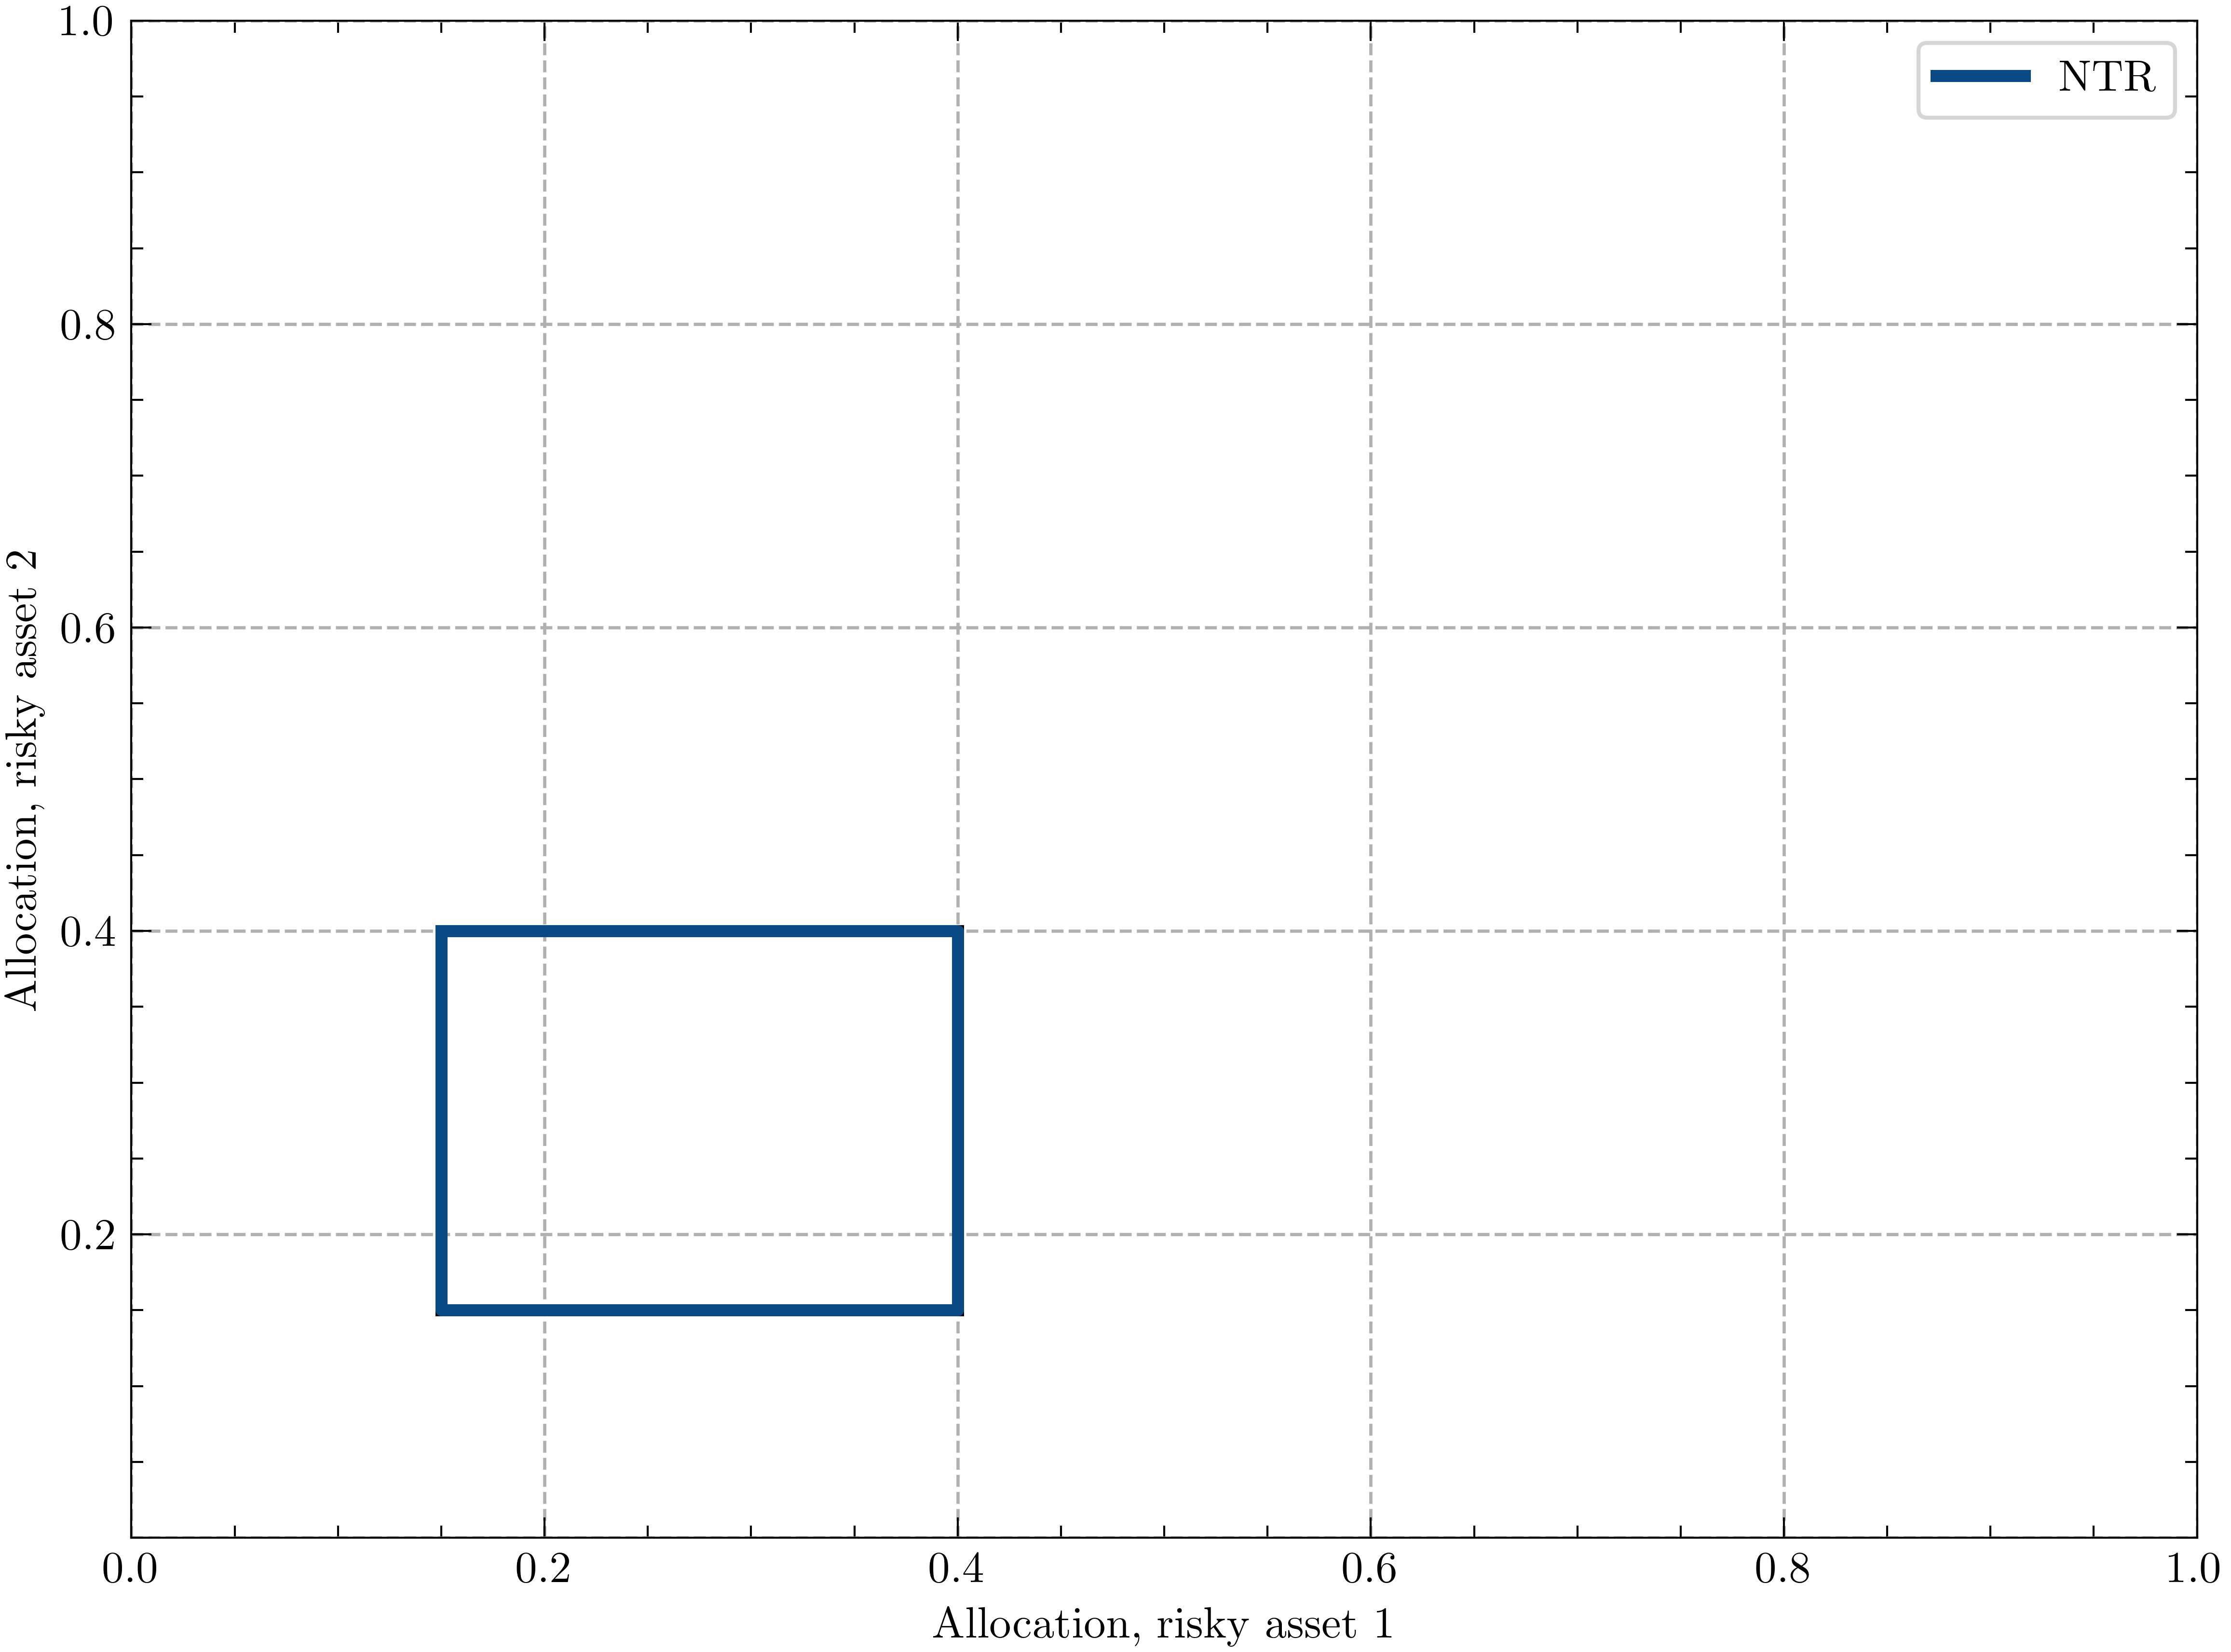
\includegraphics[scale=0.38]{Example_NTR.png}
  \end{center}
  % \floatfoot{\textbf{Note:}}
\end{figure}
The square shape of the \ac{NTR} occurs with proportional transaction costs
and independent risky assets. However the NTR is not always a square, for more on this see \textcite{Dybvig2020}.

\ifdefined\COMPILINGMAIN
% Main file is compiling this section, skip the end
\else
\printbibliography
\end{document}
\fi